\documentclass[letterpaper,10pt,draftclsnofoot,onecolumn,]{article}
% \usepackage[utf8]{inputenc}
\usepackage[margin=0.75in]{geometry}
% \usepackage{listings}
\usepackage{tikz}
% \setlengthindent{0pt}
\begin{document}
\noindent
\begin{titlepage}
    \begin{center}
        \vspace*{1cm}
        
        \textbf{Gymnastics Scoring Software}
        
        \vspace{0.5cm}
        The purpose of this paper is to define requirements for the proposed gymnastics scoring software.
        
        \vspace{1.5cm}
        
        \textbf{10.0 Software}
        
        Requirements Document\\
        CS 461\\
        Senior Software Engineering Project\\
        Fall 2018
        
    \end{center}
\end{titlepage}

\tableofcontents
\newpage

\begin{center}
\section{Introduction}
\end{center}

\subsection{System Purpose}
This system is for the scoring of gymnastics meets held in Gill Coliseum. The system will take in, calculate, organize, and display scores as well as format the scoring data.

\subsection{System Scope}
The purpose of this system is to provide an improved viewing experience for OSU Gymnastics spectators as well as making the scoring process easier for the judges. The system will comprise of a web application running on the Gill servers that is accessible by the meet staff to input or adjust scores. The scores will then be formatted to be displayed on the scoreboards inside Gill. The application will be able to format all current data into a score card that the user can print out at any time. The system will also comprise of a back-end API with a SQL database running on the Gill servers to store all scoring information.

\subsection{System Overview}
The system is comprised of three main components.
\begin{itemize}
    \item \textbf{Web Application:}
          The Web application's main function will be the user interface which allows the meet staff to add, edit and print scores. The web application will be responsible for formatting and calculating scores then pushing the data to the database and scoreboard.
    \item \textbf{Scoreboard Utilization:}
          Data collected from the web application will be pushed to display up-to-date information on current events of the meet.
    \item \textbf{Database:}
          The database will maintain information on current and past information. The information will include the teams, athletes, and the scores associated with each athlete.
\end{itemize}
\subsubsection{System Context}


\tikzset{every picture/.style={line width=0.75pt}} %set default line width to 0.75pt        

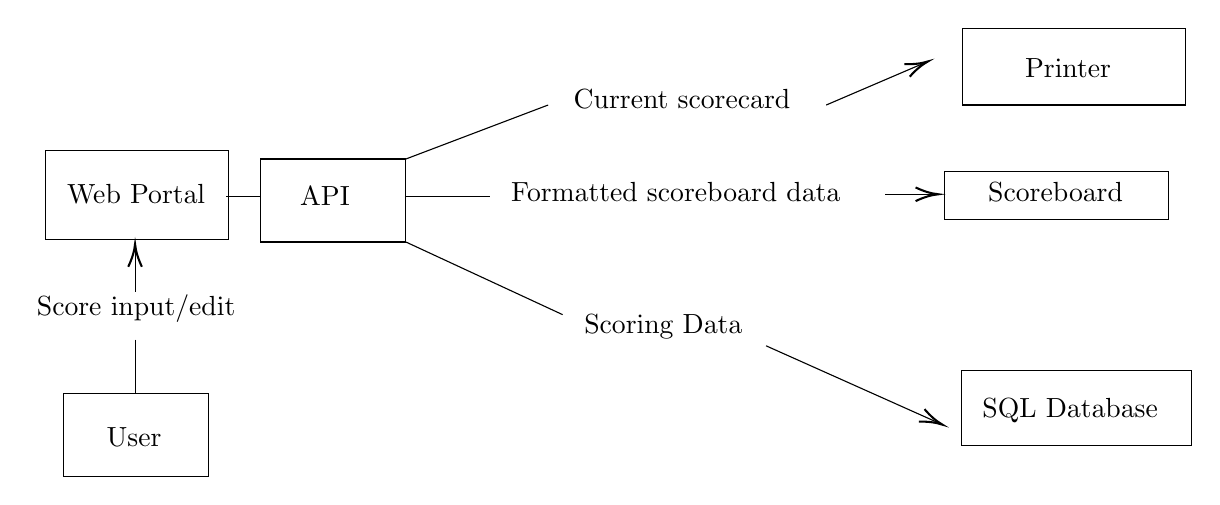
\begin{tikzpicture}[x=0.75pt,y=0.75pt,yscale=-1,xscale=1]
%uncomment if require: \path (0,300); %set diagram left start at 0, and has height of 300

%Shape: Rectangle [id:dp2117936696300492] 
\draw   (68.5,80) -- (156.5,80) -- (156.5,123) -- (68.5,123) -- cycle ;
%Shape: Rectangle [id:dp8916861139417767] 
\draw   (77,197) -- (147,197) -- (147,237) -- (77,237) -- cycle ;
%Shape: Rectangle [id:dp26609270430973364] 
\draw   (509.5,186) -- (620.5,186) -- (620.5,222) -- (509.5,222) -- cycle ;
%Shape: Rectangle [id:dp29515141413759893] 
\draw   (501.5,90) -- (609.5,90) -- (609.5,113) -- (501.5,113) -- cycle ;
%Straight Lines [id:da26603257173351713] 
\draw    (111.5,148) -- (111.5,127) ;
\draw [shift={(111.5,125)}, rotate = 450] [color={rgb, 255:red, 0; green, 0; blue, 0 }  ][line width=0.75]    (10.93,-3.29) .. controls (6.95,-1.4) and (3.31,-0.3) .. (0,0) .. controls (3.31,0.3) and (6.95,1.4) .. (10.93,3.29)   ;

%Shape: Rectangle [id:dp2818483922568308] 
\draw   (510,21) -- (617.5,21) -- (617.5,58) -- (510,58) -- cycle ;
%Straight Lines [id:da6410651706195866] 
\draw    (155.5,102) -- (171.5,102) ;


%Straight Lines [id:da027316194160433294] 
\draw    (473,101) -- (496.5,101) ;
\draw [shift={(498.5,101)}, rotate = 180] [color={rgb, 255:red, 0; green, 0; blue, 0 }  ][line width=0.75]    (10.93,-3.29) .. controls (6.95,-1.4) and (3.31,-0.3) .. (0,0) .. controls (3.31,0.3) and (6.95,1.4) .. (10.93,3.29)   ;

%Straight Lines [id:da4845127072412607] 
\draw    (242,124) -- (317.5,159) ;


%Straight Lines [id:da11103063766699672] 
\draw    (415.5,174) -- (498.67,211.18) ;
\draw [shift={(500.5,212)}, rotate = 204.09] [color={rgb, 255:red, 0; green, 0; blue, 0 }  ][line width=0.75]    (10.93,-3.29) .. controls (6.95,-1.4) and (3.31,-0.3) .. (0,0) .. controls (3.31,0.3) and (6.95,1.4) .. (10.93,3.29)   ;

%Straight Lines [id:da0750850693241939] 
\draw    (242,84) -- (310.5,58) ;


%Straight Lines [id:da18872223183152936] 
\draw    (444.5,58) -- (491.66,37.79) ;
\draw [shift={(493.5,37)}, rotate = 516.8] [color={rgb, 255:red, 0; green, 0; blue, 0 }  ][line width=0.75]    (10.93,-3.29) .. controls (6.95,-1.4) and (3.31,-0.3) .. (0,0) .. controls (3.31,0.3) and (6.95,1.4) .. (10.93,3.29)   ;

%Shape: Rectangle [id:dp7494070194947108] 
\draw   (172,84) -- (242,84) -- (242,124) -- (172,124) -- cycle ;
%Straight Lines [id:da18290866426365615] 
\draw    (111.5,171) -- (111.5,197) ;


%Straight Lines [id:da41283255297876276] 
\draw    (241.5,102) -- (282.5,102) ;



% Text Node
\draw (112,101) node  [align=left] {Web Portal};
% Text Node
\draw (111,218) node  [align=left] {User};
% Text Node
\draw (555,100) node  [align=left] {Scoreboard};
% Text Node
\draw (562,205) node  [align=left] {SQL Database};
% Text Node
\draw (112,156) node  [align=left] {Score input/edit};
% Text Node
\draw (561,40) node  [align=left] {Printer};
% Text Node
\draw (366,165) node  [align=left] {Scoring Data};
% Text Node
\draw (372,100) node  [align=left] {Formatted scoreboard data};
% Text Node
\draw (375,55) node  [align=left] {Current scorecard};
% Text Node
\draw (203,102) node  [align=left] {API};


\end{tikzpicture}

\newline
\subsubsection{System Functions}
The system's major capabilities will be managing, displaying, and exporting scores. A team score is calculated by adding the top five individual scores from that team for all four events. An individual score is given in 0.05 increments between 0 and 10 points with 10 being a perfect score. The software system should be able to drop the lowest and highest scores given for an individual if there are at least four judges. After dropping those scores, the rest should be averaged to make a final individual score. All individual scores should be sorted from highest to lowest by event regardless of team. In Gill Coliseum, there are six screens that should display the individual and team scores to the audience. Among the six screens, there are three different aspect ratios and resolutions to account for. There are five scoring tables equipped with computers including one master scoring table. Finally, the software system should be able to export the scores data. Also, the scores should be able to be printed in a readable format for the coaches, staff, and judges immediately at any time during a meet.

\subsubsection{User Characteristics}
One very important user group of the system will be the people inputting scores sitting next to the judges assigning scores to the gymnasts. The number of judges will vary between two and six. After the judges decide on the score, they will give the scores to the computer operators who will input the scores into the computers. There will be a person to input scores for each judge. In addition, there will be an information technology (IT) staff of about four people to maintain the system.


\subsection{Definitions}
All Around is all four events which is vault, bars, beam, and floor for women's gymnastics. Not all gymnasts do all four events in college gymnastics so only some gymnasts have all around scores.\\

\noindent Road to Nationals is a website that keeps all the scores for NCAA gymnastics.

% \begin{center}
% \section{References}
% \end{center}

\begin{center}
\section{System Requirements}
\end{center}

\subsection{Functional Requirements}
The system must be able to take in the number of judges from the user and have an option to drop the high and the low score. The scores given by the judges must be averaged to calculate the score for a gymnast's routine and the score for that routine will be added to the team score. There also must be an option to add exhibition routines on events that do not count towards the team score and are not displayed.\\

\noindent The system must be able to send the scores given by each judge and the final averaged score for each gymnast on each event into a database on the Gill server using SQL. The system must also be able to retrieve the scores from the database using SQL queries. The system must be able to send the data in a text file to the display boards. The display boards take care of displaying.\\

\noindent The system must be able to print out the scores at any point during the meet. The print out must include the following: each team's line up on each event, each team score for each event, all the scores from each event sorted from highest to lowest regardless of team, all the all around scores sorted from highest to lowest regardless of team, and the total team score for each team.\\

\noindent At the end of the meet, the scores must be able to be exported in the format required by Road to Nationals. These exported scores will include the same information as the printable version.\\

\noindent Making an application with different levels of authentication is a stretch goal. The fans could follow the meets with live scoring without being able to modify data or see everything that they don't need to. The staff with higher authentication could use the application to run the scoring system.

\subsection{Usability Requirements}
The user must be able to set up scoring for a meet by inputting the number of judges, choosing if scores are dropped or not, and entering the line up for each event for each team and any exhibition routines. The line ups and exhibitions can be changed throughout the meet before scores are inputted. The gymnasts doing all four events do not have to be inputted specially for all around. The system should automatically put any gymnast inputted on all four events in the all around and add up the four scores to compute the all around score. After a gymnast goes, her scores are inputted by the user and the system automatically averages the scores (dropping the high and low if that setting is on) and sends the data to a database that gets queried when needed. The displaying of scores is not automatic so that the user can decide when to display scores. The user can click an option to print out the scores at any time. At which point, the system will put the data into the printable format for the user. The user can also click to export the scores and the scores will be exported to the required format.\\

\subsection{Performance Requirements}
The performance requirements are that the system must be able to handle the maximum number of judges without errors or significant latency. The system must also be able to print out score cards during the meets without interfering with the system or significantly reducing performance.

\subsection{System Interface}
Our system will be implemented with three system interfaces, or five system interfaces if stretch goals are reached. The three main interfaces of the system are the database, the API, and the web portal. The database will be an interface used by the API to safely and securely access the data that will be used and collected by our system. Our database will be accessed using queries to multiple tables. An example query would be {\fontfamily{qcr}\selectfont SELECT COUNT(*) players FROM oregonstate} which would hypothetically grab all of the players from the oregonstate table and return the results for use by our API. Continuing, the API will be an interface for the web portal to send CRUD commands to the API that will then do the difficult work of handling the data. Lastly, the web portal is the interface for users to access the API in an easily usable manner. The web portal will require the user to select the gymnast performing, the event the gymnast performed, and their score and send that to the API. The last two interfaces would consist of an iOS and Android app that would provide users with live scores.

\subsection{System Operations}
There are multiple operations that our system must be able to perform, and the operations can be broken down three ways: database operations, API operations, and client operations. \\

\noindent To start, the database will have to be able to create, read, update, and delete data. These are known as CRUD operations and are common practice when using databases. \\

\noindent Next, are the operations that need to be performed by the API which are much more involved. The API will need to be able to take in data in the form of JSON, and from there the API will have to parse the JSON for three major things: authentication, data, and command. This is the cornerstone operation of our server. After receiving and parsing the data, the API will have to be able to handle three major operations: printing the current score sheet, updating the display boards, and processing the score. Printing the score sheet will consist of the API grabbing the current data of the meet, formatting it into a pdf, and then sending the pdf to a printer. Updating the display boards will consist of the API grabbing the most recently processed team scores, the current gymnast, and the current event then formatting the data into a text document and sending that text document to the display boards. The last operation will consist of the API performing calculations on the scores sent in, followed by updating the team scores, and then querying the database to add the new scores to the correct player and updating the team scores.  \\

\noindent The last set of operations are the client operations. These will be performed by the web portal that users interact with. Only three operations are needed to be done by the web portal; these operations are handling log ins, setting up a meet, and sending scores. Due to the security concern and the want for data to only be handled by trust worthy sources, the web portal will require users to provide a user name and password to prove their identity as a non malicious agent. The next operation is setting up a meet, this will involve choosing the number of judges and teams in each meet. After the number of judges and teams have been chosen, the operation will then prompt the user for the names of the teams participating and the players participating for each team. For sending scores, the application will allow for users to choose the team and player, and from there the user will be able to insert the scores from each judge then send the scores to the API.

\subsection{System Modes and States}
The modes for the system are different numbers of judges and dropping the high and the low score or not. If there are three or less judges, dropping the high and the low score is not an option since there wouldn't be anything left to average. The system states include the input gathered from the user for setup, the inputted scores from the user, and the scores calculated and put into the database.\\

\subsection{Physical Characteristics}
Our program will require the physical requirements of a server that can run a SQL database, display screens, and at least one web enabled device. The server will need to be able to run a containerized API with a SQL server attached. The display screens will need to be able to take in a text document of information that will be displayed to the screens, and lastly, the web enabled devices will need to be able to access a web page.

\subsection{Environmental Conditions}
Our environment will primarily be Gill Coliseum, which is a weather controlled indoor environment. The hardware that needs to be used is also already housed in Gill Coliseum allowing for easy access for both software and hardware. Overall, the environment will not pose an issue for our project.

\subsection{System Security}
System security will be implemented using CIA security principles. Starting with Confidentiality we plan on implementing our API using HTTPS protocols that protect data being sent over the internet. Moreover, we plan to store our data in a SQL database that can only be accessed by specific administrators. Next, in order to ensure the data is not tampered with we will be implementing different levels of users. The base level will be allowed to read team scores and individual scores of players, whereas administrator level accounts will have the ability to access the create, update, and delete functions of our API. Lastly, we plan to keep our data and API available by keeping it on a private wifi network that will avoid the traffic from users at the gymnastics meets to ensure that we do not lose packets due to throughput. Another plan is the stretch goal of rate limiting, which will help protect the API from Denial of Service attacks.

\subsection{Information Management}
We will be collecting data from the organizers of the gymnastics meets that the software will be used with. The data will be sent by the teams, judge's assistants, and organizers. The teams will send their active roster, the judge's assistants will send their scores for each event, and the organizer will send data about the date and location of the event. The data will be sent over HTTPS standards to a local server that will be set up by the organizer. Each local server will have a local SQL database that will store all of the information needed, and this database will only be accessible by a root user that is created by the API allowing only the API, and the organizers of the event to be able to directly access the database. At the end of each meet, the scores will be sent to Road to Nationals which is an organization that stores and compiles gymnastics scores from across the nation.

\subsection{Policies and Regulations}
This section is intentionally left blank so we can check with the sponsor to make sure there are no Oregon State University, NCAA, or Federal policies or regulations that we have to follow for potential protections of student athletes.

\begin{center}
\section{Verification}
\end{center}
The client will verify that the system meets the requirements by running a mock meet that goes through all the steps of a regular meet for the scoring system. After going through the scoring of a mock meet, the client and our team will decide if the software meets each of the requirements listed in this requirements document. We will also decide if any stretch goals were met but those are not necessary for the system to be functional. \\

\begin{center}
\section{Appendices}
\end{center}

\subsection{Assumptions and Dependencies}
Some assumptions that our team is making is that the hardware provided by Gill, such as the scoreboard or server, are adequate in terms of performance and no major work will need to be done upgrading these hardware components.

\subsection{Acronyms and Abbreviations}
API: Applied Programming Interface\newline
CIA: Confidentiality Integrity Availability\newline
CRUD: Create Read Update Delete\newline
HTTP: Hyper Text Transfer Protocol\newline
HTTPS: Hyper Text Transfer Protocol Secure\newline
NCAA: National Collegiate Athletics Association\newline
OSU: Oregon State University\newline
SQL: Structured Query Language\newline

\end{document}
